\chapter{Inflation} \label{ch:vi}

The first few sections of this chapter aren't directly related to inflation, but are useful tools that will allow us to address some of the problems brought about by the standard (non-inflationary) cosmological model.

\section{Luminosity Distance}

If the redshift is not very small, we have to think more carefully about what we mean by "distance" in cosmology. The instantaneous physical distance (proper distance) is a convenient construct, but not itself observable, since observation always refer to our past light cone. In Euclidean space, there are a number of different ways to infer the distance of an object, for example comparing its apparent brightness to its intrinsic luminosity.
\par In a Euclidean space, we could define the \emph{luminosity distance} as
\begin{equation*}
    d_{L} = \left(\frac{L}{4\pi F}\right)^{1/2}
\end{equation*}
with intrisic luminosity $L$ and measured flux $F$. But how does this change in a curved and expanding Universe, and why?
\par For two reasons mainly:
\begin{enumerate}
    \item \emph{Geometry}: The space is no longer Euclidean, and the surface of the 2-sphere onto which the luminosity is diluted is $4\pi a_{0}^{2}\tilde{r}_{s}^{2} = 4\pi a_{0}^{2}f_{k}(\chi)^{2}$, where $f_{k}(\chi)$ is 
    \begin{equation}
        \chi = \int_{0}^{r_{s}}\frac{\diff{r}}{\sqrt{1-kr^{2}}} = f_{k}^{-1}(r_{s}) = \left\{
            \begin{array}{ll}
                r_{s} & k=0\\
                \arcsin(r_{s}) & k=1\\
                \text{arcsinh}(r_{s}) & k=-1
            \end{array}
        \right.
    \end{equation}
    \item \emph{Correction to the concept of luminosity}: In an expanding Universe, we have to be a little more cautious, and the necessary steps to be taken are explained in detail in the following.
\end{enumerate}
\par Because of the expansion, the wavelength of these photons will change according to (\ref{eq:redshift_def}). Therefore, the energy of a photon will decrease
\begin{equation*}
    E_{0} \sim \frac{c}{\lambda_{0}} = \frac{c}{(1+z)\lambda_{e}} \sim \frac{E_{e}}{1+z}
\end{equation*}
\par On top of that, two wavefronts separated by $\delta t_{e}$ will arrive with a delay $\delta t_{0} = \delta t_{e}(1+z)$, so the arrival rate will decrease of another $1+z$
\begin{equation*}
    L_{e} \sim \frac{E_{e}}{\delta t_{e}} = \frac{(1+z)^{2}E_{0}}{\delta t_{0}} = (1+z)^{2}L_{0}
\end{equation*}
\par Since the flux is equal to energy per unit time per unit area, we can write
\begin{equation*}
    F = \frac{L_{e}}{4\pi a_{0}^{2}\tilde{r}_{s}^{2}(1+z)^{2}} = \frac{L_{e}}{4\pi a_{0}^{2}f_{k}(\chi)^{2}(1+z)^{2}}
\end{equation*}
so that by direct comparison with out initial equation, we find that the \emph{luminosity distance} is
\begin{equation}
    d_{L} = a_{0}\tilde{r}_{s}(1+z) = (1+z)a_{0}f_{k}(\chi)
    \label{eq:luminositydistance}
\end{equation}
\par The luminosity distance is something we might hope to measure, since there are some astrophysical sources whose absolute luminosity are known, but $\chi$ (and, for extension, the comoving distance $\tilde{r}_{s}$), is not directly observable, so we have to remove it from our equation. On a null radial geodesic (for convenience), we have
\begin{equation*}
    0 = \text{d}s^{2} = -\text{d}t^{2} + a^{2}\text{d}\chi^{2}
\end{equation*}
or more simply 
\begin{equation*}
    \chi = \int \frac{\text{d}t}{a} = \int \frac{\text{d}a}{a^{2}H(a)}
\end{equation*}
\par It is conventional to convert the scale factor to redshift using (\ref{eq:scalefactor_redshift}) $a = a_{0}(1+z)^{-1}$, so we have
\begin{equation*}
    \chi(z) = \int_{0}^{z}\frac{\text{d}z'}{a_{0}H(z')}
\end{equation*}
\par In order to evaluate the Hubble parameter in this integral we can use Friedmann equation (\ref{eq:friedmann_alt}), thus finding 
\begin{equation*}
    d_{L}(z) = (1+z)a_{0}f_{k}\left[a_{0}^{-1}H_{0}^{-1}\int_{0}^{z} \frac{\text{d}z'}{E(z')}\right]
\end{equation*}
where we've defined $E(z) = H(z)/H_{0}$. Still, it is more common to speak in terms of $\Omega_{c,0} = -k/a_{0}^{2}H_{0}^{2}$, which can be measured. We can therefore write the luminosity in terms of measurable cosmological parameters as 
\begin{equation}
    \boxed{
    d_{L}(z) = (1+z)\frac{H_{0}^{-1}}{\sqrt{|\Omega_{c,0}|}}f_{k}\left[\sqrt{|\Omega_{c,0}|}\int \frac{\text{d}z'}{E(z')}\right]
    }
    \label{eq:general_lumdist}
\end{equation} \marginpar{Recall that the spatial density parameter $\Omega_{c,0}$ must abide the consistency relation $$ 1 = \sum_{i}\Omega_{i,0} + \Omega_{c,0} $$}
\par Although it appears unwieldy (and it kinda is), this equation is of central importance in cosmology. Given the observables $H_{0}$ and $\Omega_{i,0}$, we can straightforwardly calculate the luminosity distance to an object at any redshift $z$.
\begin{figure}[h!]
    \centering 
    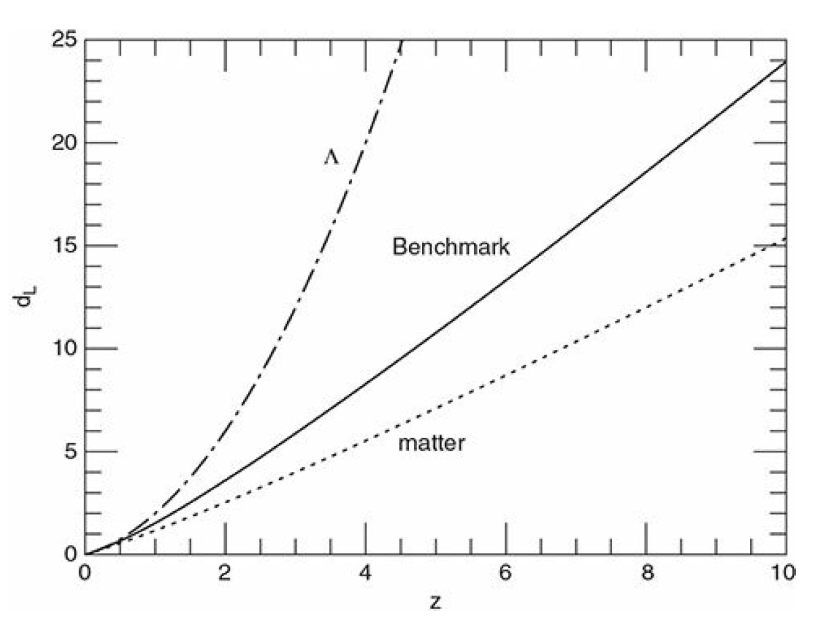
\includegraphics[width=0.9\textwidth]{img/lumdist.png}
    \caption{Luminosity distance of a standard candle with observed redshift $z$, in units of the Hubble distance, $c/H_{0}$. The bold solid line gives the result for the Benchmark Model. For comparison, the dot-dash line indicates a flat, $\Lambda$-dominated Universe, and the dotted line a flat, matter-dominated Universe.}
    \label{fgr:lumdist}
\end{figure}
\par Experimentally, it's more common to use a quantity known as \emph{distance module} to quantify distances. It is related to the luminosity distance through the definition of absolute magnitude
\begin{equation}
    \mu = 5\log_{10}\left(\frac{d_{L}}{10\unit{pc}}\right)
    \label{eq:distancemodule}
\end{equation}
Remarkably, going back in time (so at higher redshift) we observe a change in the slope of the luminosity distance curve (or, equivalently, of the distance module) at roughly $z = 0.5$ caused by the change from an accelerating Universe ($\Lambda$DU) to a decelerating Universe (MDU).
\par If we define $z_{\Lambda}$ the redshift at which there is equivalence between the $\Lambda$ and matter density parameters 
\begin{equation}
    \Omega_{\Lambda,0} = \Omega_{m,0}(1+z_{\Lambda})^{3} \implies z_{\Lambda} = \left(\frac{\Omega_{\Lambda,0}}{\Omega_{m,0}}\right)^{1/3}-1
\end{equation}
we find it to be $z_{\Lambda}\approx 0.44$, which is the exact cause of the \href{https://en.wikipedia.org/wiki/Cosmic_coincidence_problem}{\emph{cosmic coincidence problem}}, since it appears rather odd that the Cosmological Constant is dominating at a redshift so "close" to present time.

\section{Second Order Hubble Law}

If you recall, earlier we've defined Hubble-Le Maître's law (\ref{eq:hubblelaw}) at the linear order. It is the purpose of this section to stretch our approximation a bit further, including larger redshifts and, by extension, a second-order correction to the aforementioned law.
\par Let us now approximate $a(t)$ in a neighborhood of today
\begin{equation*}
    a(t) = a(t_{0}) + \left(\parder{a}{t}\right)_{t_{0}}(t-t_{0}) + \frac{1}{2}\left(\parparder{a}{t}\right)_{t_{0}}(t-t_{0})^{2} + \text{o}\left((t-t_{0})^{3}\right)
\end{equation*}
so that
\begin{equation}
    a(t) = a_{0}\left[1 + H_{0}(t-t_{0})-\frac{1}{2}q_{0}H_{0}^{2}(t-t_{0})^{2} + \text{o}\left((t-t_{0})^{3}\right)\right]
    \label{eq:a_expansion-second}
\end{equation}
where we've defined 
\begin{equation}
    H_{0} = \left(\frac{\dot{a}(t)}{a(t)}\right)_{t_{0}} \quad q_{0} = -\left(\frac{\ddot{a}(t)a(t)}{\dot{a}^{2}(t)}\right)_{t_{0}}
\end{equation}
\par We also know that
\begin{equation*}
    z = \frac{a(t_{0})}{a(t)}-1 \approx -1 + \frac{1}{1-H_{0}(t_{0}-t)-\frac{1}{2}H_{0}^{2}q_{0}(t_{0}-t)^{2}}
\end{equation*}
We can find an approximate relation for the redshift Taylor expanding its definition
\begin{equation*}
    z \approx H_{0}(t_{0}-t)+\left(1+\frac{q_{0}}{2}\right)H_{0}^{2}(t_{0}-t)^{2}
\end{equation*}
\par Remember that at first order we found the relation $z(t) = H_{0}(t_{0}-t)$, which we can plug into last equation introducing corrections only to the third order
\begin{equation}
    H_{0}(t_{0}-t) \approx z(t) -\frac{1}{2}(q_{0}+2)z^{2} +\text{o}(z^{3})
\end{equation}
\par Now we'll turn to investigate how all of this enters into the definition of proper distance
\begin{equation}
    \tilde{r}_{s} =  \int_{0}^{r_{s}}\frac{\diff{r}}{\sqrt{1-kr^{2}}} = \int_{t_{e}}^{t_{0}}\frac{\diff{t}}{a}
\end{equation}
where we're considering a null, radial geodesic for the FLRW metric (\ref{eq:FRW}). We can plug in the second order expansion for $a(t)$
\begin{equation}
    \tilde{r}_{s} = \frac{1}{a_{0}}\int_{t_{e}}^{t_{0}}\diff{t}\left[1+H_{0}(t_{0}-t)+\frac{1}{2}H_{0}^{2}q_{0}(t_{0}-t)^{2}\right]^{-1}
\end{equation}
We can neglect the third-order contribution brought by the third term in the right-hand side of the equation and expand once more 
\begin{equation}
    \tilde{r}_{s} \approx \frac{1}{a_{0}}\int_{t_{e}}^{t_{0}}\diff{t}\left[1-H_{0}(t_{0}-t)\right] = \frac{(t_{0}-t_{e})}{a_{0}} - \frac{H_{0}(t_{0}-t_{e})^{2}}{2a_{0}}
\end{equation}
which means that our proper distance is ($c=1$)
\begin{equation}
    \tilde{r}_{s} = \frac{1}{a_{0}}\left[(t_{0}-t_{e})+\frac{1}{2}H_{0}(t_{0}-t_{e})^{2}\right]
\end{equation}
or, in terms of the redshift and reintroducing the missing $c$ factors
\begin{equation}
    \tilde{r}_{s}(t_{0}) = \frac{c}{H_{0}}z\left[1-\frac{(1+q_{0})}{2}z\right]
    \label{eq:properdistance_rs_second}
\end{equation}
We can substitute the expression at second order for the proper distance in the definition of distance luminosity (\ref{eq:luminositydistance}) to find 
\begin{equation}
    d_{L}^{2} = \frac{1}{H_{0}^{2}}\left(z-\frac{1}{2}(q_{0}+2)z^{2}+\frac{z^{2}}{2}\right)^{2}(1+z)^{2}
\end{equation}
which we can expand to quadratic order 
\begin{equation}
    H_{0}d_{L} = -\left[z-\frac{1}{2}(q_{0}+1)z^{2}\right](1+z) = z+z^{2}-\frac{1}{2}(q_{0}+1)z^{2} + \text{o}(z^{3})
\end{equation}
which yields
\begin{equation}
    \boxed{
    H_{0}d_{L} = z + \frac{1}{2}(1-q_{0})z^{2} + \text{o}(z^{3})
    }
\end{equation}

\section{Angular diameter distance}

\par Let's consider a curved, expanding Universe described by the FLRW metric and choose your comoving coordinate system so that the observer is at its origin.
\par Consider a yardstick of constant proper length $l$ perpendicular to the line of sight and at a comoving coordinate distance $r_{e}$. At a time $t_{e}$, the yardstick emitted the light that you observe at time $t_{0}$. The comoving coordinates of the two ends of the yardstick, at the time the light was emitted, were $(r_{e},\theta_{1},\varphi)$ and
$(r_{e},\theta_{2},\varphi)$.
\par The distance $\text{d}s$ between the two ends of the yardstick, measured at the time $t_{e}$ when the light was emitted, can be found from the FLRW metric
\begin{equation*}
    \text{d}s = a(t_{e})f_{k}(\chi)\diff{\Omega} = a(t_{e})\tilde{r}_{s}\diff{\Omega}
\end{equation*}
where $a(t_{e})\tilde{r}_{s}$ is the physical (proper) distance of the emitter at the time of emission. We can set $\text{d}s = l$ and define
\begin{equation}
    d_{A} := \frac{\diff{s}}{\diff{\Omega}} = \tilde{r}_{s}\frac{a(t_{e})}{a_{0}}a_{0} = \frac{\tilde{r}_{s}a_{0}}{(1+z)}
\end{equation}
from which we conclude
\begin{equation}
    d_{A} = \frac{a_{0}f_{k}(\chi)}{1+z} = \frac{d_{L}}{(1+z)^{2}}
    \label{eq:angulardistance}
\end{equation}
You can also show that 
\begin{align*}
    H_{0}d_{A} &= \left[z-\frac{1}{2}(1-q_{0})z^{2}+\text{o}(z^{3})\right](1-2z+\text{o}(z^{2}))\\
    &= z-\frac{1}{2}(3+q_{0})z^{2}+\text{o}(z^{3})
\end{align*}
which is the Hubble law as a function of the angular distance.
\par We can define the apparent brightness $B$ as 
\begin{equation}
    B = \frac{l}{\Omega} = \frac{L}{4\pi d_{L}^{2}}\frac{d_{A}^{2}}{S}
    \label{eq:apparentbrightness}
\end{equation}
where $l$ is the apparent luminosity, $\Omega$ is the angular extension, and $S$ is the physical extension of the source. We can further manipulate the definition introducing the absolute luminosity per unit area, which depends only on the intrinsic characteristic of the source 
\begin{equation}
    B = \frac{\mathcal{L}}{4\pi}\left(\frac{d_{A}}{d_{L}}\right)^{2} = \frac{\mathcal{L}}{4\pi}(1+z)^{-4}
\end{equation}
Suppose that the redshift we observe were produced by some absorbing medium between us and the object. In an Euclidean Universe
\begin{equation}
    d_{L} = d(1+z)^{1/2}
\end{equation}
while $d_{A} = d$, and so 
\begin{equation}
    \frac{d_{A}}{d_{L}} = \frac{1}{(1+z)^{1/2}} \implies B \propto (1+z)^{-1}
\end{equation}
but (un)fortunately observations are telling us that $B \propto (1+z)^{-4}$, thus allowing us to discard the scenario in which the redshift is wholly produced by absorbing media (rather than an expanding Universe).

\section{Particle Horizon}

Consider a photon emitted by some source at time $t_{e}$, for a light path $\text{d}s = 0$. The maximum comoving distance the photon might have travelled to present day is
\begin{equation}
   a^{-1}(t)\diff{t} = \frac{\diff{r}}{\sqrt{1-kr^{2}}} \implies \int_{0}^{t_{0}}\frac{\diff{t}}{a(t)} = \int_{0}^{d_{H}}\frac{\diff{r}}{\sqrt{1-kr^{2}}}
\end{equation}
For a single component (flat) Universe, the expression for $a(t)$ is simple
\begin{equation}
    a(t) \propto t^{n} \quad n = \frac{2}{3(1+w)}
\end{equation}
and the integral is well defined provided that $n < 1$, which implies $w > -1/3$ in the EoS of the Cosmological fluid (accelerating Universe). The maximum (physical) distance travelled by a photon is then defined as 
\begin{equation}
    d_{\text{max}} = R_{H}(t_{0}) = a(t_{0})\int_{0}^{t_{0}}\frac{\diff{t}}{a(t)} = a(t_{0})\tilde{r}_{\text{max}}(t_{0})
\end{equation}
Such distance is commonly known as \emph{particle horizon} and represents the maximum distance from which we might have possibly received information from the past via electromagnetic waves. For a flat Universe ($k=0$) \marginpar{Recall the definition of $x$ $$ x = \frac{a(t)}{a_{0}} = \frac{1}{1+z(t)}$$}
\begin{equation}
    \diff{t} = \frac{\diff{x}}{xH_{0}E(x)} \implies d_{\text{max}}(t_{0}) = \int_{0}^{1}\frac{\diff{x}}{H_{0}xE(x)}
\end{equation}
while for a "standard" single-component Universe
\begin{equation}
    R_{H}(t) = a(t)\int_{t_{i}}^{t}\frac{\diff{t'}}{a(t')} \quad a(t)\propto t^{n}
\end{equation}
which is also equal to ($t \gg t_{i}$)
\begin{equation}
    R_{H}(t) = t^{n}\left[\frac{1}{1-n}t^{1-n}\right]^{t}_{t_{i}} \approx \frac{t}{1-n}
\end{equation}
We might relate this last result to the Hubble radius $H^{-1}$, obtaining
\begin{equation}
    \frac{H^{-1}}{R_{H}} = \frac{1-n}{n}
\end{equation}
but please note that this last equation holds only for a simple cosmological model with a single dominating component.

\subsubsection{Event Horizon}

We define the \emph{event horizon} as the maximum distance at which an object can be so that a signal emitted by that same object reaches us at a future infinite. Fixed an emission time $t_{\star}$
\begin{equation}
    \int_{t_{\star}}^{\infty}\frac{\diff{t}}{a(t)} = \int_{0}^{r_{\star}}\frac{\diff{r}}{\sqrt{1-kr^{2}}}
\end{equation}
If $r_{s} < r_{\star}$, the event will never be observed, meaning there could be regions of spacetime that are impossible to "communicate" with. To see if the integral can actually be finite, you will usually check \marginpar{We're assuming a flat Universe $k=0$ for which $$ a(t) = A e^{Ht}$$}
\begin{equation}
    r_{\star} = -\frac{1}{AH}e^{-Ht}\Big|^{\infty}_{t_{\star}} < \infty
\end{equation}
For example, if the EoS has $w>-1/3$, $r_{\star}\to \infty$ and the horizon is not properly defined.

\section{Flatness Problem}

Consider a Universe with vanishing Cosmological Constant $\Lambda = 0$ which is also such that Einstein's equation is \emph{always} valid, also at $t=0$. If we define
\begin{equation}
    \Omega_{k} = 1-\Omega = \frac{\rho_{c}-\rho}{\rho_{c}} = -\frac{k}{a^{2}H^{2}}
\end{equation}
Now assume that $k\neq 0$ and $\Omega_{k}$ can evolve independently from the dominant contribution to the cosmological fluid. If
\begin{itemize}
    \item MDU: $a(t)\propto t^{2/3}$ and $H \propto a^{-3/2} \implies \Omega_{k}\sim a \sim t^{2/3}\sim \Gamma^{-1}$;
    \item RDU: $a(t)\propto t^{1/2}$ and $H \propto a^{-2} \implies \Omega_{k}\sim a^{2} \sim t \sim \Gamma^{-2}$.
\end{itemize}
Going back in time has the effect of decreasing the value of $\Omega_{k}$. Through studies of the CMB (see Chapter \ref{ch:v} for more), the Planck collaboration managed to put bounds to the value of $\Omega_{k}$, which was found to be
\begin{equation}
    |\Omega_{k}(t_{0})| < 0.05
\end{equation}
At the time of matter-radiation equality, the spatial density parameter was 
\begin{equation}
    \Big| \frac{\Omega_{k}(t_{eq})}{\Omega_{k}(t_{0})}\Big|^{-1} = \frac{T_{eq}}{T_{0}} \sim 10^{4} \implies |\Omega_{k}(t_{eq})| < 10^{-4}
\end{equation}
Similarly, if we extrapolate backward to the time of Big Bang nucleosynthesis, at $a_{BBN} \approx 3.6\cdot 10^{-9}$
\begin{equation*}
    |1-\Omega_{BBN}|<7\cdot10^{-16}
\end{equation*}
and the distance from unity would only decrease if we went even further back in time. Setting then those orders of magnitude as initial conditions imply a \emph{huge fine-tuning problem}.
\par There is no known reason for the density of the Universe to be so close to the critical density, and this appears to be an unacceptably strange coincidence in the view of most astronomers and cosmologists. This is the so called \emph{Flatness problem}.
\par Let us define 
\begin{equation}
    x = \log\left(\frac{a}{a_{0}}\right) \implies H = \der{\ln(a)}{t} \implies \diff{t} = \frac{1}{H}\diff{\ln(a)} = \frac{1}{H}\diff{x}
\end{equation}
and recall Friedmann equation (\ref{eq:friedmann1}) for a perfect fluid
\begin{equation}
    \frac{\ddot{a}}{a} = -\frac{4\pi G}{3}\rho (1+3w) \implies 2q = (1+3w)\Omega(t)
\end{equation}
and by direct substitution you can check that 
\begin{equation}
    \frac{\dot{H}}{H^{2}} = -(1+q)
\end{equation}
Putting all of this to work, we gather 
\begin{equation}
    \der{\Omega_{k}}{t} = \frac{k}{a^{3}}\frac{2\dot{H}}{H^{3}} + \frac{k}{H^{2}}\frac{2\dot{a}}{a^{3}} = -2\Omega_{k}H\left(1+\frac{\dot{H}}{H^{2}}\right) = -2\Omega_{k}H(1-(1+q))
\end{equation}
If we want the final result to be independent from the particular cosmology that we've chosen \marginpar{Just in case you have forgotten, with the superscript we're referring to the derivative with respect to the conformal time.}
\begin{align}
    & \Omega_{k}' = 2\Omega_{k}q \\
    & 2q = (1+3w)\Omega = (1+3w)(1-\Omega_{k})
\end{align}
which means 
\begin{equation}
    \boxed{
        \Omega_{k}' = (1+3w)(1-\Omega_{k})\Omega_{k}
    }
\end{equation}
This tells us that if $\Omega_{k}\approx 0$, the stationary point is unstable if $1+3w > 0$! Similarly, $\Omega_{k}\approx 0$ is a stable attractor if $1+3w < 0$, which means $w < -1/3$.
\par The flatness problem is thus resolved if we postulate a Universe that accelerates for enough time. Such period of time is called \emph{inflationary epoch} or just \emph{inflation}.
\par If during the inflation $H \sim \text{const,}$ then 
\begin{equation}
    \Omega_{k} \approx -\frac{k}{a^{2}H^{2}}
\end{equation}
Let $t_{i}$ be inflation's starting time and $t_{f}$ the ending time
\begin{equation}
    \frac{\Omega_{k}(t_{f})}{\Omega_{k}(t_{i})} = \left(\frac{a_{f}}{a_{i}}\right)^{2} = e^{-2N}
\end{equation}
where we defined $N = \ln(a_{f}/a_{i})$ the number of $e$-folds of the inflationary epoch. We want that at the end of inflation $|\Omega_{k}(t_{f})|\sim 10^{-61}$, while we assume a strongly non-flat Universe at the beginning of inflation $|\Omega_{k}(t_{i})|\sim 1$. For our requirements to be met, the Universe should expand a number of $e$-folds such that
\begin{equation}
    e^{-2N} \approx 10^{-60} \implies N \geq 60
\end{equation}
During inflation, then, the comoving Hubble radius is decreasing 
\begin{equation}
    \boxed{
    \frac{1}{aH} \downarrow \implies |\Omega_{k}| = \frac{|k|}{a^{2}H^{2}}\downarrow
    }
    \label{eq:solvedfp}
\end{equation}
thus resulting in a quasi-de Sitter Universe with $p=-\rho$ and $H \sim \text{const.}$

\section{Horizon Problem}

Another problem remains to be addressed. We know that photons decouple from ordinary matter at $z\approx 1100$ (decoupling/last scattering). Currently, within our particle horizon, we observe a roughly homogeneous temperature distribution, which is that of the CMB. So far so good.
\par From last scattering until present day, the Universe was dominated by non-relativistic matter, hence 
\begin{equation}
    R_{H}(t_{LS})\approx H_{LS}^{-1} = H_{0}^{-1}\left(\frac{a_{LS}}{a_{0}}\right)^{3/2}\approx R_{H}(t_{0})\left(\frac{a_{LS}}{a_{0}}\right)^{3/2}
\end{equation}
But here comes the problem. 
\par Since 
\begin{quote}
    \begin{center}
        "\emph{Scales scale with the scale factor}"
    \end{center}
\end{quote}
meaning \marginpar{This is essentially the corresponding particle wavelength at last scattering.}
\begin{equation} 
    \lambda_{H_{0}}(t_{LS}) = \frac{R_{H}(t_{0})}{1+z_{LS}}
\end{equation}
we get a gargantuan problem $R_{H}(t_{LS}) \ll \lambda_{H_{0}}(t_{LS})$, which can be rewritten in a perhaps clearer form 
\begin{equation}
    \left(\frac{\lambda_{H_{0}}(t_{LS})}{R_{H}(t_{LS})}\right)^{3} = \left(\frac{a_{LS}}{a_{0}}\right)^{-3/2} \approx 10^{5}
\end{equation}
which means that $10^{5}$ volumes are \emph{not} in causal connection!
\begin{figure}[h!]
    \centering
    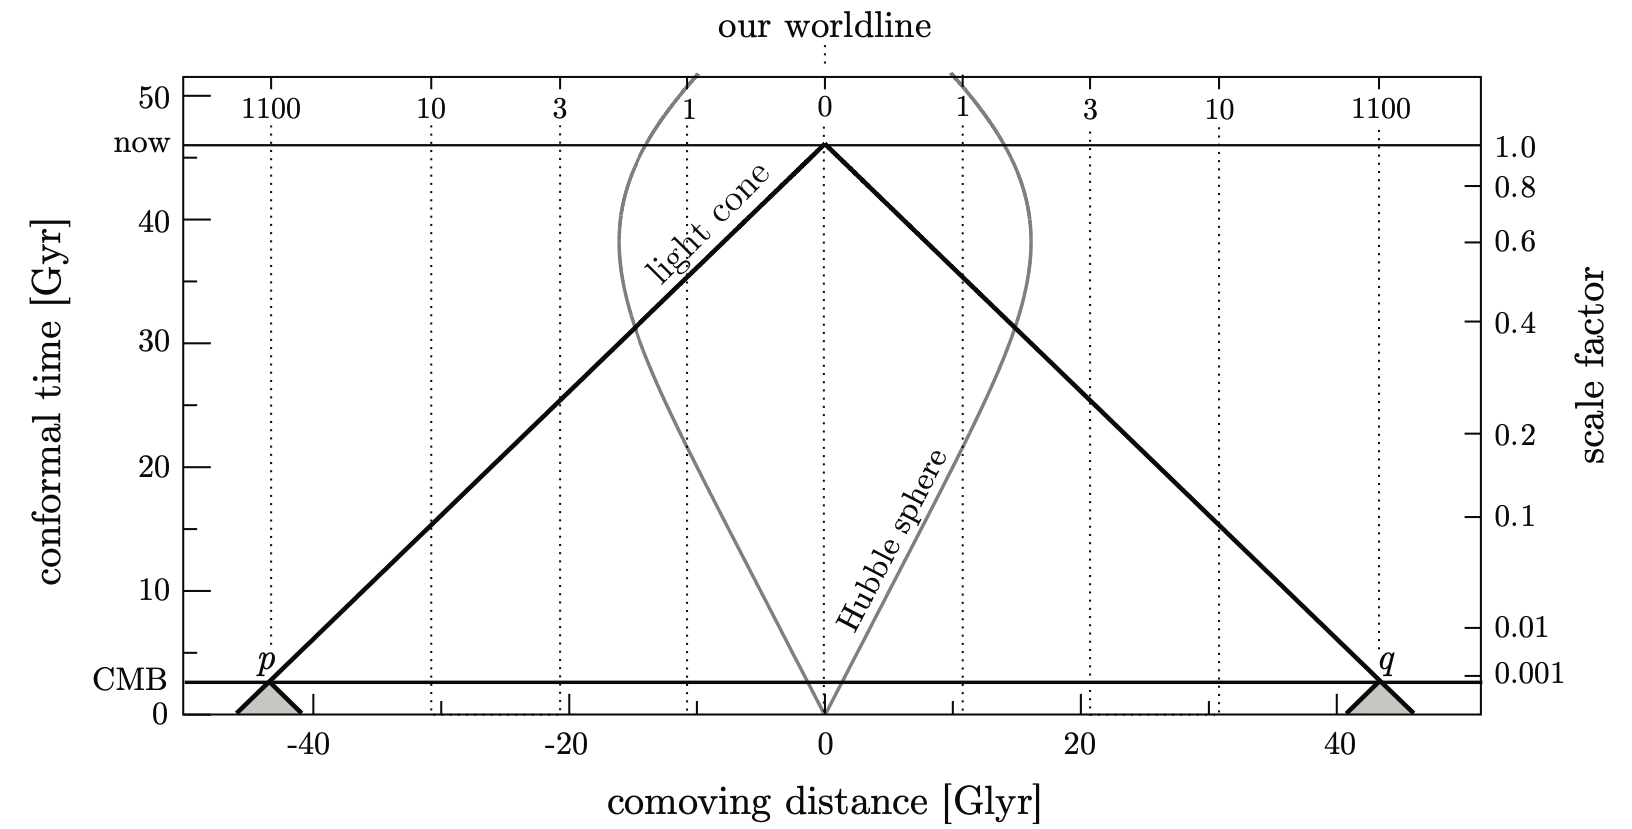
\includegraphics[width=0.8\textwidth]{img/hp.png}
    \caption{The horizon problem in the conventional Big Bang model. All events that we currently observe are on our past light cone. The intersection of our past light cone with the spacelike slice labelled CMB corresponds to two opposite points in the observed CMB. Their past light cones don’t overlap before they hit the singularity, $a = 0$, so the points appear never to have been in causal contact. The same applies to any two points in the CMB that are separated by more than 1 degree on the sky. Credits: \cite{Baumann_2022}.}
    \label{fgr:hp}
\end{figure}
\par This is a huge problem in order to find a sensible explanation for the impressive homogeneity of the CMB (since after decoupling photons are no longer interacting with matter).
\par Perhaps you won't be surprised when I say that inflation comes to the rescue this time as well.
\par During inflation $H_{i}^{-1}\approx \text{const,}$ while structures continue to grow until they eventually cross the horizon. If we assume a large enough inflationary period, the scales within which we observe the current homogeneity could be able to enter once more into the horizon because they're exponentially suppressed.
\par At the end of an à la de Sitter inflation (but French-sounding) the particle horizon was 
\begin{equation}
    R_{H} = a_{f}\int_{t_{i}}^{t_{f}}\frac{\diff{t}}{a(t)}
\end{equation}
with 
\begin{equation}
    a(t) = a(t_{i})\exp(H_{i}(t-t_{i}))
\end{equation}
meaning that 
\begin{equation}
    \frac{a_{f}}{a_{i}} = \frac{a(t_{f})}{a(t_{i})} = \exp(H_{i}(t_{f}-t_{i}))
\end{equation}
We can also invert the expression
\begin{equation}
    a(t_{i}) = a(t_{f})\exp(-H_{i}(t_{f}-t_{i}))
\end{equation}
and define the number of $e$-folds like we've done earlier $N = H_{i}(t_{f}-t_{i})$. This allows us to write 
\begin{equation}
    R_{H}(t_{f}) = a(t_{f})\int_{t_{i}}^{t_{f}} \frac{\diff{t}}{a(t_{f})}\exp(H_{i}(t_{f}-t))
\end{equation}
If we assume that the particle horizon at last scattering is such that 
\begin{equation}
    R_{H}(t_{LS}) = a(t_{LS})\int_{t_{i}}^{t_{LS}}\frac{\diff{t}}{a(t)} \approx a(t_{LS})\int_{t_{i}}^{t_{f}}\frac{\diff{t}}{a(t)}\exp(H_{i}(t_{f}-t))
\end{equation}
we conclude 
\begin{equation}
    \boxed{
        R_{H}(t_{LS}) = \frac{a_{LS}}{a(t_{f})}\frac{1}{H_{i}}\left[\exp(H_{i}(t_{f}-t_{i}))-1\right] = \frac{a_{LS}}{a(t_{f})}\frac{1}{H_{i}}(e^{N}-1)
    }
\end{equation}
\par Our problem is solved if $R_{H}(t_{LS}) > \lambda_{H_{0}}(t_{LS})$
\begin{equation}
    \frac{a_{LS}}{a(t_{f})}\frac{1}{H_{i}}(e^{N}-1) > \frac{1}{H_{0}(1+z_{LS})} = \frac{a_{LS}}{a_{0}H_{0}}
\end{equation}
hence if
\begin{equation}
    \boxed{
        e^{N} \gtrsim \frac{a(t_{f})H_{i}}{a(t_{0})H_{0}}
    }
    \label{eq:solvedhp}
\end{equation}
How do we interpret this last result? All scales we observe today had always been causally connected during the whole expansion of the Universe.
\par For the sake of completeness, let's prove that the conditions to solve both the flatness and horizon problems are the same.
\begin{equation}
    |\Omega_{k}(t_{0})| = \frac{|k|}{a_{0}^{2}H_{0}^{2}} \quad |\Omega_{k}(t_{f})| = \frac{|k|}{a_{f}^{2}H^{2}(t_{f})}
\end{equation}
This implies \marginpar{Recall that during inflation the Hubble constant is not changing.}
\begin{equation}
    |\Omega_{k}(t_{0})|a_{0}^{2}H_{0}^{2} = |\Omega_{k}(t_{f})|a_{f}^{2}H^{2}(t_{f}) = |\Omega_{k}(t_{f})|a_{f}^{2}H_{i}^{2}
\end{equation}
but 
\begin{equation}
    \Big|\frac{\Omega_{k}(t_{f})}{\Omega_{k}(t_{i})}\Big| = e^{-2N} \implies |\Omega_{k}(t_{0})| = e^{-2N}|\Omega_{k}(t_{i})|\left(\frac{a_{f}^{2}H_{i}^{2}}{a_{0}^{2}H_{0}^{2}}\right)
\end{equation}
If we set $|\Omega_{k}(t_{i})| \approx 1$ \marginpar{The request $|\Omega_{k}(t_{0})| < 1$ purely relies on observational evidence and on (\ref{eq:densityparam_eq}).}
\begin{equation}
    |\Omega_{k}(t_{0})|\approx e^{-2N}\left(\frac{a_{f}^{2}H_{i}^{2}}{a_{0}^{2}H_{0}^{2}}\right) < 1 \iff e^{N} > \frac{a(t_{f})H_{i}}{a_{0}H_{0}}
\end{equation}
which is the condition that solves the horizon problem.
\begin{figure}[h!]
    \centering 
    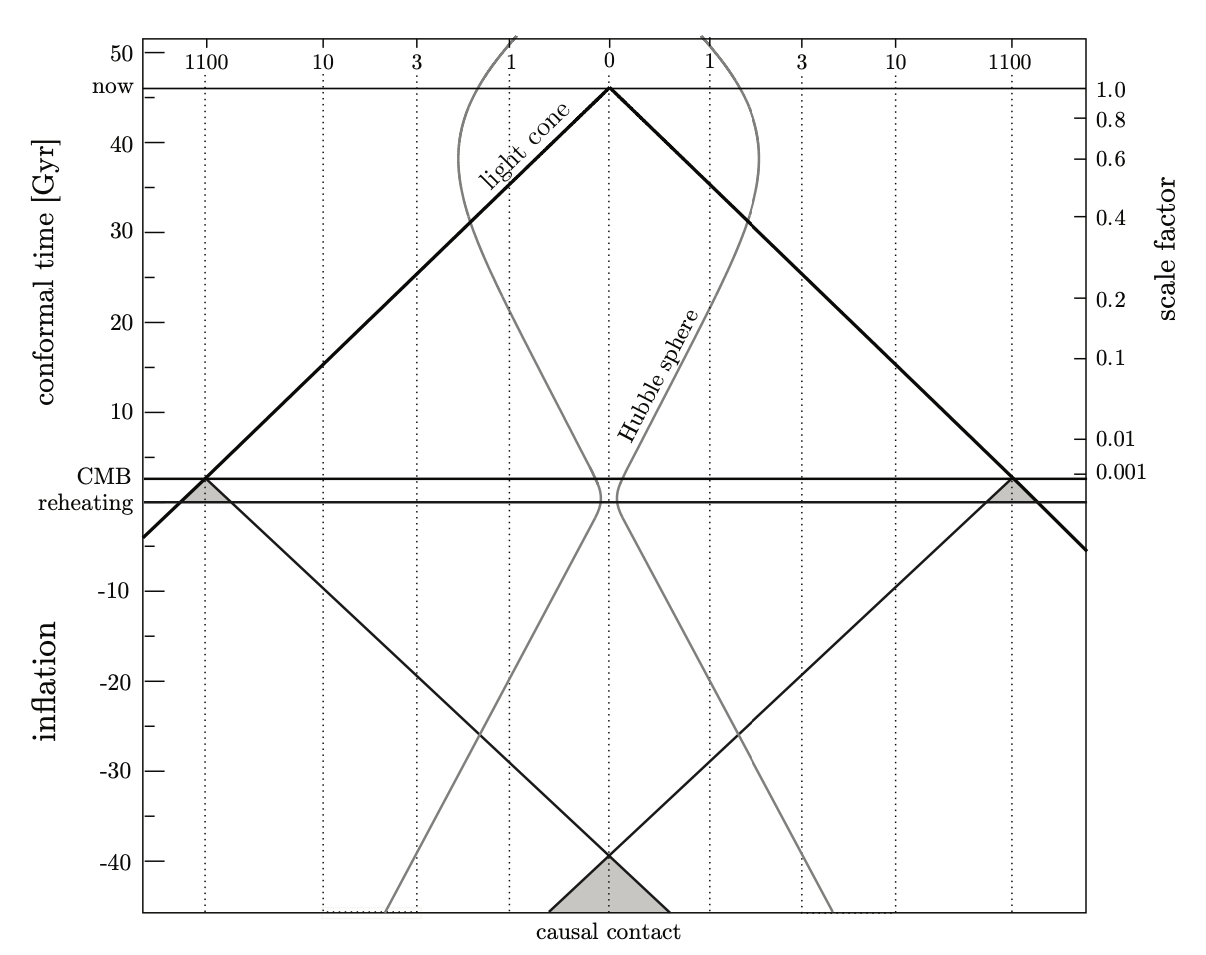
\includegraphics[width=0.8\textwidth]{img/hpinflation.png}
    \caption{Inflationary solution to the horizon problem. The comoving Hubble sphere shrinks during inflation and expands during the conventional Big Bang evolution (at least until dark energy takes over at $a \approx 0.5$). Conformal time during inflation is negative. The spacelike singularity of the standard Big Bang is replaced by the reheating surface, i.e. rather than marking the beginning of time it now corresponds simply to the transition from inflation to the standard Big Bang evolution. All points in the CMB have overlapping past light cones and therefore originated from a causally connected region of space. Credits: \cite{Baumann_2022}.}
    \label{fgr:hpinflation}
\end{figure}

\section{Hubble Radius}

The Hubble radius we've defined as $R_{H}\sim H^{-1}$ for both MDU and RDU is different from that we have in an accelerated Universe. The Hubble radius at a given time $t$ is roughly equal to the distance travelled by a photon during an "expansion time," (the time needed for the scale parameter to double) starting from said time $t$.
\par As a consequence, two particles that are separated by $\lambda > H^{-1}(t_{0})$ will also be causally connected if the distance that separated them at some earlier time was $\lambda(t) < H^{-1}(t)$.
\par Say that $\tilde{R}_{H}(t_{0})$ is the distance crossed by a photon in $t \to t_{\star}$ so that $a(t_{\star}) = 2a(t)$ (so, an expansion time). By virtue of its own definition
\begin{equation}
    \tilde{R}_{H}(t) = a(t_{\star})\int_{t}^{t_{\star}} \frac{\diff{t}}{a(t)} = a(t_{\star})\int_{a(t)}^{a(t_{\star})}\frac{\diff{a}}{a^{2}H} = a(t_{\star})\int_{a(t)}^{2a(t)}\frac{\diff{a}}{a^{2}H}
\end{equation}
\par Consider a small expansion time (respect to the age of the Universe) so that approximately $H(t)\sim\text{const.}$ Then
\begin{equation}
    \tilde{R}_{H}(t) = \frac{1}{H(t)}
\end{equation}
but if now $\lambda < H_{0}^{-1}$, while $\lambda > H(t_{LS})^{-1}$ at an earlier time, then there must necessarily exist an epoch during which $\lambda$ is growing faster than $H^{-1}$
\begin{equation}
    \frac{\text{d}}{\text{d}t}\left(\frac{\lambda}{H^{-1}}\right) > 0
\end{equation}
but if $\lambda \sim a$, this implies $\ddot{a} > 0$, hence the Universe must be accelerating, hence the necessity of inflation.
\par What we surmise, then, is that the comoving Hubble radius $(aH)^{-1}$ must be increasing right after the BBN, but for earlier times it must be decreasing, as pictorially shown in Fig.\ref{fgr:inflation}.
\begin{figure}[h!]
    \centering 
    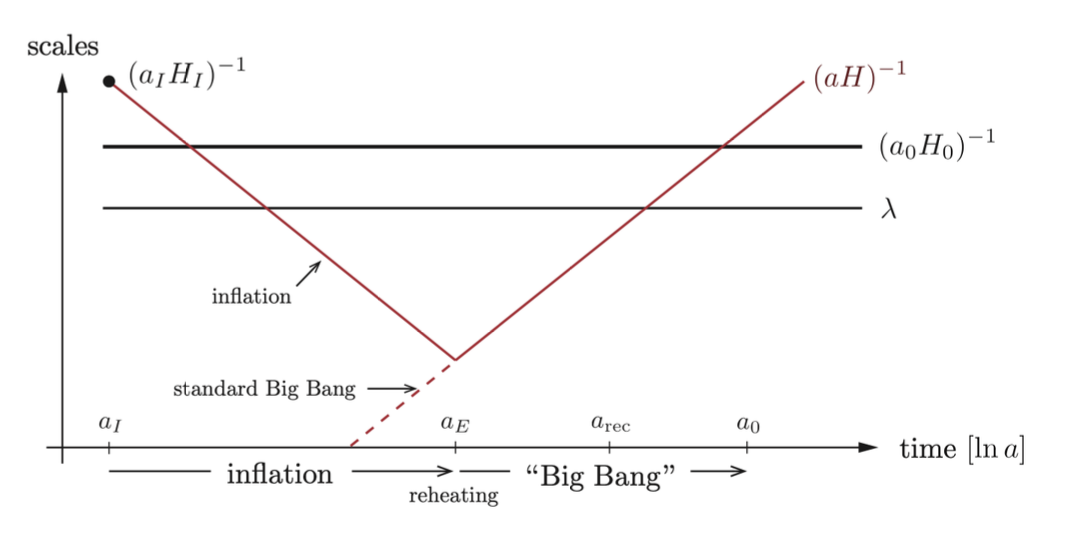
\includegraphics[width=0.75\textwidth]{img/inflationscales.png}
    \caption{Scales of cosmological interest were larger than the Hubble radius until $a \approx 10^{-5}$ (where today is at $a(t_{0}) = 1$). However, at very early times, before inflation operated, all scales of interest were smaller than the Hubble radius and therefore susceptible to microphysical processing. Notice the symmetry of the inflationary solution. Scales just entering the horizon today, 60 $e$-folds after the end of inflation, left the horizon 60 $e$-folds before the end of inflation. Credits: \cite{Baumann_2022}.}
    \label{fgr:inflation}
\end{figure}
\par The existence of an epoch of accelerated expansion corresponds to having $p < -\rho/3$ and violates the \emph{strong energy condition}.
\par Several cosmologists began to postulate the necessity of an inflationary period starting from the end of 1970s. Remarkably, Starobinski{\v{i}} \cite{1979JETPL..30..682S} noted that quantum corrections to GR should be important for the early Universe.
\par The solution to the Einstein field equations in the presence of curvature squared terms, when the curvatures are large, leads to an effective Cosmological Constant. Therefore, he proposed that the early Universe went through an inflationary de Sitter era, but never mentioned that such inflationary epoch could solve the problems intrinsic of the standard hBBN model.
\par Only two years later, Guth \cite{1981PhRvD..23..347G}, and the following month still Guth and Weinberg \cite{1981PhRvD..23..876G}, showed that the horizon and flatness problems could be solved if we allowed the existence of an extraordinary supercooling in the early history of the Universe to temperatures 28 or more orders of magnitude below the critical temperature for some phase transition. But
\begin{quote}
    \begin{center}
        \emph{"Unfortunately, the scenario seems to lead to some unacceptable consequences, so modifications must be sought."}
    \end{center}
\end{quote}
\begin{figure}[h!]
    \centering 
    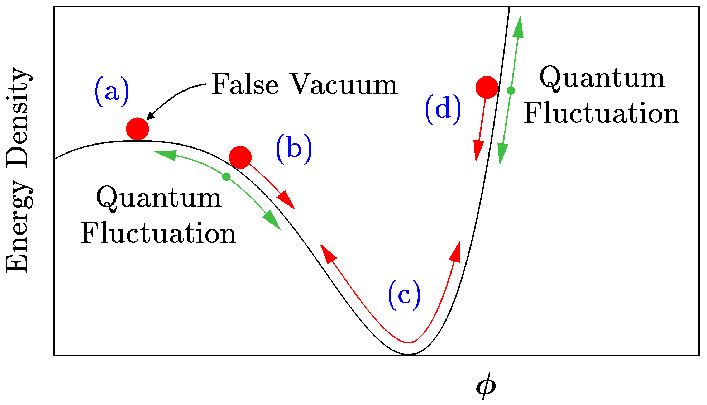
\includegraphics[width=0.7\textwidth]{img/guthinflation.jpg}
    \caption{In simple inflationary models, the Universe at early times is dominated by the potential energy density of a scalar field, $\varphi$. Red arrows show the classical motion of $\varphi$. When $\varphi$ is near region (a), the energy density will remain nearly constant, $\rho\approx \rho_{f}$, even as the Universe expands. Moreover, cosmic expansion acts like a frictional drag, slowing the motion of $\varphi$: Even near regions (b) and (d), $\varphi$ behaves more like a marble moving in a bowl of molasses, slowly creeping down the side of its potential, rather than like a marble sliding down the inside of a polished bowl. During this period of "slow roll," $\rho$ remains nearly constant. Only after $\varphi$ has slid most of the way down its potential will it begin to oscillate around its minimum, as in region (c), ending inflation. Credits: \href{https://ned.ipac.caltech.edu/level5/March05/Guth/Guth1.html}{this website}.}
\end{figure}
\par In short, they were postulating the existence of a scalar field $\varphi$. The associated potential $U(\varphi)$ had to present a local maximum where the phase transition occurred (so at the beginning of inflation), and a local minimum where $U(\varphi)\approx \text{const.} = \Lambda$, hence a metastable de Sitter phase during which tunnel effect occurred towards true vacuum. This was the so-called \emph{old inflation}.
\par What had gone wrong with Guth's and Weinberg's model was solved only one year later by Andrej Dmitrievič Linde \cite{1982PhLB..108..389L}, \cite{1982PhLB..116..335L} and independently by Andreas Albrecht and Paul Steinhardt \cite{1982PhRvL..48.1220A} in a model named \emph{new inflation} or \emph{slow-roll inflation}.
\par In this model, instead of tunneling out of a false vacuum state, inflation occurred by a scalar field rolling down a potential energy hill. When the field rolls very slowly compared to the expansion of the Universe, inflation occurs. However, when the hill becomes steeper, inflation ends and reheating can occur.
\begin{figure}[h!]
    \centering 
    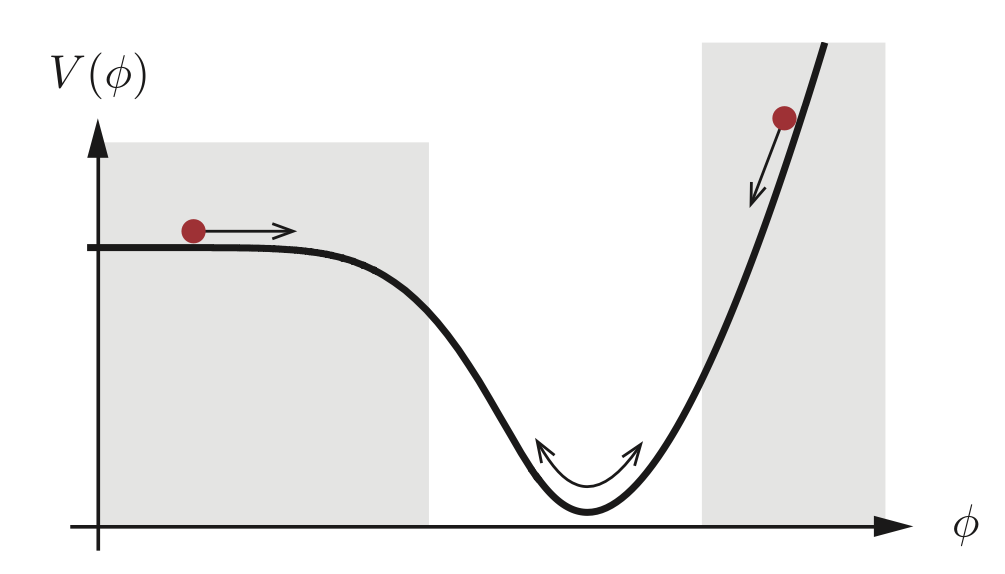
\includegraphics[width=0.7\textwidth]{img/slowroll.png}
    \caption{Example of a slow-roll potential as postulated by Linde, Albrecht, and Steinhardt. Inflation occurs in the shaded parts of the potential. Credits: \cite{Baumann_2022}.}
    \label{fgr:slowroll}
\end{figure}

\section{Slow-roll Inflation}

Let's consider an inflationary model as brought about by a scalar field $\varphi$ we will call, in a very witty fashion, \emph{inflaton}. To the scalar field $\varphi$ is associated an action $S$
\begin{equation}
    S = \int \text{d}^{4}x \sqrt{-g}\mathcal{L} = \int \text{d}^{4}x \sqrt{-g}\left[\frac{1}{2}g^{\mu\nu}\partial_{\mu}\varphi\partial_{\nu}\varphi - V(\varphi)\right]
    \label{eq:inflatonaction}
\end{equation}
where $\sqrt{-g} = a^{3}$ for the FLRW metric (\ref{eq:FRW}). We can calculate Euler-Lagrange equations
\begin{equation}
    \partial^{\mu}\frac{\delta(\sqrt{-g}\mathcal{L})}{\delta(\partial^{\mu}\varphi)} - \frac{\delta(\sqrt{-g}\mathcal{L})}{\delta\varphi} = 0
\end{equation}
which yield \marginpar{Note the presence of a Hubble-friction term $3H\dot{\varphi}$ that we wouldn't have in a static Universe.}
\begin{equation}
    \ddot{\varphi} + 3H\dot{\varphi} - \frac{\nabla^{2}\varphi}{a^{2}}+V'(\varphi) = 0 \quad V'(\varphi) = \der{V(\varphi)}{\varphi}
\end{equation}
Consider also the energy-momentum tensor associated to the action $S$ (\ref{eq:inflatonaction}), which we can obtain simply variating the action with respect to the metric 
\begin{equation}
    T_{\mu\nu} = \frac{2}{\sqrt{-g}}\frac{\delta(\sqrt{-g}\mathcal{L})}{\delta g_{\mu\nu}}
    \label{eq:generalemtensor}
\end{equation}
obtaining
\begin{equation}
    T_{\mu\nu} = \partial_{\mu}\varphi\partial_{\nu}\varphi -g_{\mu\nu}\mathcal{L}
\end{equation}
We can give a little twist to this last expression so that it looks like the energy-momentum tensor of a perfect fluid 
\begin{equation}
    T^{\mu\nu} = p_{\varphi}g^{\mu\nu} + (p_{\varphi}+\rho_{\varphi})u^{\mu}u^{\nu}
\end{equation}
where $\rho_{\varphi}$ and $p_{\varphi}$ are respectively
\begin{align}
    \rho_{\varphi} &= T^{00} = \frac{\dot{\varphi}^{2}}{2} + V(\varphi) + \frac{(\nabla\varphi)^{2}}{2a^{2}}\\
    p_{\varphi} &= \frac{T^{ii}}{3} = \frac{\dot{\varphi}^{2}}{2}-V(\varphi)-\frac{(\nabla\varphi)^{2}}{6a^{2}}
\end{align}
\par If the field is strongly dishomogeneous and, as a consequence, $|\nabla\varphi|$ is large
\begin{align}
    \rho_{\varphi} &\approx + \frac{(\nabla\varphi)^{2}}{2a^{2}}\\
    p_{\varphi} &\approx -\frac{(\nabla\varphi)^{2}}{6a^{2}}
\end{align}
which means 
\begin{equation}
    p_{\varphi} \approx - \frac{1}{3}\rho_{\varphi}
\end{equation}
and hence $w = -1/3$. However, a Universe so dishomogeneous cannot give raise to an inflationary epoch. So let's consider instead a scalar field that is decomposed as 
\begin{equation}
    \varphi(\vec{x},t) = \varphi_{0}(t) + \delta\varphi(\vec{x},t)
\end{equation}
where the former term is that associated to a "classical" field ($\lambda \to \infty$), while the latter is associated to quantum fluctuations. If we assume the quantum fluctuations to be negligible respect to the classical field $\delta\varphi \ll \varphi_{0}$, we can neglect the contribution brought by $\delta\varphi$ to the evolution (\emph{back-reaction}). Hence
\begin{align}
    T^{00} &= \rho_{\varphi} = \frac{\dot{\varphi}_{0}^{2}}{2} + V(\varphi_{0})\\
    \frac{T^{ii}}{3} &= p_{\varphi} = \frac{\dot{\varphi}_{0}^{2}}{2} - V(\varphi_{0})
\end{align}
which grants $p_{\varphi} \approx - \rho_{\varphi}$, thus producing a pseudo-de Sitter evolution. The equation of motion then turns into
\begin{equation}
    \boxed{
        \ddot{\varphi}_{0} +3H\dot{\varphi}_{0} + V'(\varphi_{0}) = 0
    }
    \label{eq:inflatoneom}
\end{equation}
which is the Klein-Gordon equation for the inflaton. In the limit $V(\varphi_{0}) \gg \dot{\varphi}_{0}^{2}/2$, the scalar field is "slowly-rolling" in the potential. And this is all thanks to the friction term!
\par The 2nd Friedmann equation (\ref{eq:friedmann2}) for the background density is 
\begin{equation}
    H^{2} = \frac{8\pi G}{3}\left(\frac{1}{2}\dot{\varphi}^{2}+V(\varphi)\right)
    \label{eq:fried_altalt}
\end{equation}
which we can differentiate with respect to time to yield 
\begin{equation}
    2H\dot{H} = \frac{8\pi G}{3}\left(\dot{\varphi}\ddot{\varphi}+\der{V}{\varphi}\dot{\varphi}\right) = -8\pi G H \dot{\varphi}^{2}
\end{equation}
ultimately leading to 
\begin{equation}
    \boxed{
        \dot{H} = -4\pi G \dot{\varphi}^{2}
    }
    \label{eq:hdot}
\end{equation}
\par From the first Friedmann equation, on the other hand, we have 
\begin{align*}
    \frac{\ddot{a}}{a} = -\frac{4\pi G}{3}(\rho + 3p) &= -\frac{4\pi G}{3}(2\dot{\varphi}^{2}-2V(\varphi)) \\
    &= -\frac{4\pi G}{3}\left[3\dot{\varphi}^{2} -2\left(\frac{1}{2}\dot{\varphi}^{2}+V(\varphi)\right)\right]
\end{align*}
so that recalling (\ref{eq:fried_altalt}), (\ref{eq:hdot}), the 1st Friedmann equation is rewritten as
\begin{equation}
    \frac{\ddot{a}}{a} = \dot{H} + H^{2}
\end{equation}
and we can define the 1st slow-roll parameter $\varepsilon$
\begin{equation}
    \boxed{
        \varepsilon = -\frac{\dot{H}}{H^{2}}
    }
    \label{eq:slowroll1}
\end{equation}
so that \marginpar{Note that more than one slow-roll parameter exist, but only the first, $\varepsilon$, determines the inflation.}
\begin{equation}
    \frac{\ddot{a}}{a} = (1-\varepsilon)H^{2}
\end{equation}
and the Universe is accelerating only if $\varepsilon < 1$. If we now request the Universe to be (ideally) a pseudo-de Sitter with $H\approx \text{const}$, we can consider the relative variation $\dot{H}/H$ over an Hubble time ($H^{-1}$) and require 
\begin{equation}
    \Big|\frac{\dot{H}}{H}\frac{1}{H}\Big| \ll 1 \implies |\varepsilon|\ll 1
\end{equation}
In terms of the number of $e$-folds from the beginning of inflation up to time $t$ we can also write
\begin{equation}
    \varepsilon = -\der{\ln (H)}{N} \quad N = \log\left(\frac{a(t)}{a_{i}}\right)
\end{equation}
which also means $\diff{N} = H\diff{t}$ and 
\begin{equation}
    -\frac{\dot{H}^{2}}{H^{2}} = -\der{\ln(H)}{N}
\end{equation}
The 1st slow-roll parameter $\varepsilon$ thus describes, in some sense, the displacement from a purely de Sitter Universe.
\par Let's now show that $\varepsilon \ll 1 \iff V(\varphi) \gg \dot{\varphi}^{2}/2$
\begin{align*}
    (\implies) \quad -\dot{H} = 4\pi G \dot{\varphi}^{2} \ll H^{2} &= \frac{8\pi G}{3}\left(\frac{1}{2}\dot{\varphi}^{2}+V(\varphi)\right) \\
    & \implies \dot{\varphi}^{2}\ll V(\varphi)
\end{align*}
which is the first direction of the implication. Let's now prove that the reverse holds as well
\begin{equation}
    (\impliedby) \quad p\approx -\rho \to
    \left\{
        \begin{array}{ll}
            \dot{\rho} +3H(p+\rho) = 0 & \implies \dot{\rho}\approx 0\\
            H^{2} \approx \frac{8\pi G}{3}\rho & \implies H^{2} \approx \text{const.}
        \end{array}
    \right.
\end{equation}
and at this point concluding is trivial $H^{2} \approx \text{const.} \implies H \approx \text{const} \implies \varepsilon \ll 1$.
\par Let's define the \emph{second slow-roll parameter} $\delta$ (dimensionless acceleration per Hubble time)
\begin{equation}
    \boxed{
        \delta = -\frac{\ddot{\varphi}}{H\dot{\varphi}}
    }
    \label{eq:slowroll2}
\end{equation}
and require it to be $\delta \ll 1$. This is because the variation of $\varepsilon$ during an $e$-fold must be small, and so 
\begin{equation}
    \der{\varepsilon}{N} = \frac{1}{H}\der{\varepsilon}{t} = \frac{1}{H}\left(-\frac{\ddot{H}}{H^{2}}+\frac{2\dot{H}^{2}}{H^{3}}\right) = -\frac{\dot{H}}{H^{2}}\left(\frac{\ddot{H}}{H\dot{H}}-2\frac{\dot{H}}{H^{2}}\right)
\end{equation}
which implies \marginpar{You can prove the last equality directly substituting from $-\dot{H} = 4\pi G \dot{\varphi}^{2}$}
\begin{equation}
    \frac{1}{\varepsilon}\der{\varepsilon}{N} = \left(\frac{\ddot{H}}{H\dot{H}}-2\frac{\dot{H}}{H^{2}}\right) \implies \frac{\ddot{\varphi}}{H\dot{\varphi}} = |\delta| \ll 1
\end{equation}
\par So far, no approximations have been made. We simply noted that in a regime where $\{\varepsilon, |\delta|\} \ll 1$, inflation occurs and persists. We now use these conditions to simplify the equations of motion. This is called the slow-roll approximation. The condition $\varepsilon \ll 1$ implies $V(\varphi) \gg \dot{\varphi}^{2}/2$ and hence leads to the following simplification of the Friedmann equation
\begin{equation}
    \boxed{
    H^{2} \approx \frac{8\pi G}{3}V(\varphi)
    }
    \label{eq:slowrollfriedmann}
\end{equation}
In the slow-roll approximation, the Hubble expansion is determined completely by the potential energy. The condition $|\delta| \ll 1$ then simplifies the Klein-Gordon equation (\ref{eq:inflatoneom}) to
\begin{equation}
    \dot{\varphi} \approx -\frac{V'(\varphi)}{3H} \textoversymbol{=}{\varepsilon \ll 1} -V'\left[24\pi G V(\varphi)\right]^{-1/2}
\end{equation}
This provides a simple relationship between the gradient of the potential and the speed of the inflaton. This is the so-called $\alpha$-\emph{relation}
\begin{equation}
    \boxed{
    \dot{\varphi} \approx -\frac{V'}{\sqrt{24 \pi G V(\varphi)}}
    }
    \label{eq:alpharel}
\end{equation}
Moreover, if $\epsilon,\,\delta \ll 1$
\begin{equation}
    \epsilon = -\frac{\dot{H}}{H^{2}} = \frac{4\pi G \dot{\varphi}^{2}}{\frac{8\pi G}{3}V(\varphi)} \approx \frac{1}{16\pi G}\left(\frac{V'(\varphi)}{V(\varphi)}\right)^{2}
\end{equation}
where we've introduced the $\alpha$-relation in the last equality. This leads to the \emph{first flatness condition}
\begin{equation}
    \boxed{
    \Big|\frac{V'(\varphi)}{V(\varphi)}\Big| \ll \sqrt{16\pi G}
    }
    \label{eq:flatness1}
\end{equation}
Consider now 
\begin{equation}
    \ddot{\varphi} = -\frac{\text{d}}{\text{d}t}\left(\frac{V'}{3H}\right) \implies \ddot{\varphi} = -\frac{V''\dot{\varphi}}{H} + \frac{V'\dot{H}}{3H^{2}}
\end{equation}
which, requiring $\epsilon,\,\delta \ll 1$, yields
\begin{equation}
   \ddot{\varphi} = -\frac{V''}{3H}\left(-\frac{V'}{3H}\right) + \frac{V'}{3}\left(\frac{1}{16\pi G}\frac{V'^{2}}{V^{2}}\right) \quad \frac{V'}{3}\left(\frac{1}{16\pi G}\frac{V'^{2}}{V^{2}}\right) \ll \frac{V'}{3}
\end{equation}
Hence, since 
\begin{equation}
    |\ddot{\varphi}| \ll |H\dot{\varphi}| = \frac{1}{3}|V'(\varphi)|
\end{equation}
we conclude 
\begin{equation}
    \Big|\frac{V''}{3H}\Big|\cdot \Big|\frac{V'}{3H}\Big| \ll \frac{V'}{3}
\end{equation}
which also means $|V''|\ll 3H^{2}$, thus leading us to the \emph{second flatness condition}
\begin{equation}
    \boxed{
    \Big|\frac{V''(\varphi)}{V(\varphi)}\Big| \ll 8\pi G
    }
    \label{eq:flatness2}
\end{equation}
When both flatness conditions hold, the expansion of the Universe is exponential (pseudo-de Sitter) and is also exponentially long. The inflation epoch will end only when, at a certain time $t_{f}$, the first slow-roll parameter is $\varepsilon = 1$
\begin{equation}
    N(\varphi) = \ln\left(\frac{a(t_{f})}{a(t)}\right) = \int_{t}^{t_{f}}H\diff{t} = \int_{\varphi}^{\varphi_{f}}\frac{H}{\dot{\varphi}}\diff{\varphi}
\end{equation}
which, after requiring $\epsilon,\,\delta \ll 1$, turns into 
\begin{equation}
     N(\varphi) \approx \int_{\varphi}^{\varphi_{f}}\left[\frac{8\pi G V}{3}\frac{24\pi G V}{V'^{2}}\right]^{1/2}\diff{\varphi}
\end{equation}
The number of $e$-folds from the end of inflation starting from an arbitrary time $t$ is then 
\begin{equation}
    \boxed{
    N(\varphi) = 8\pi G \int_{\varphi}^{\varphi_{f}}\frac{V}{V'}\diff{\varphi}
    }
    \label{eq:efolds}
\end{equation}
\par The first flatness condition told us that 
\begin{equation}
    \Big|\frac{V}{V'}\Big| \gg (16\pi G)^{-1/2}
\end{equation}
which allows us to constrain (\ref{eq:efolds})
\begin{equation}
    N(\varphi) = 8\pi G \int_{\varphi}^{\varphi_{f}}\frac{V}{V'}\diff{\varphi} \gg \sqrt{4\pi G}|\varphi_{f}-\varphi|
\end{equation}
Hence the number of $e$-folds for our inflationary model will always be
\begin{equation}
    N \gg \sqrt{4\pi G}|\varphi_{f}-\varphi_{i}|
\end{equation}
which, in principle, we can invert to find the range spanned by the scalar field $\varphi$
\begin{equation}
    \Delta\varphi \ll \frac{N}{\sqrt{4\pi G}}
\end{equation}
with the minimum number of $e$-folds necessary to replicate the current Universe ($N_{\text{min}} \approx 60$), the estimated upper bound for the field variation is $\Delta\varphi \ll 10^{20}\unit{GeV}$.
\begin{flushright}
    \emph{The End.}
\end{flushright}